\section{Implementation}

\subsection{SketchImporter}

For the implementation of the SketchImporter component two classes were created: The \textit{BackgroundImageTool} and the \textit{ZeroPointMoveAction}. The second one is just a helper class which is used by the other to move the imported image to the "`zero point"' (0,0) and therefore extends the abstract \textit{MoveAction}.
The \textit{BackgroundImageTool} extends the \textit{ImageTool}-class provided by JHotDraw. The basic image import is already implemented there. The imported image is only moved to the right location and set as background. Therefore the \textit{DrawingView} has to be used, which could be accessed through the \textit{getView} method.

\begin{figure}[h]
    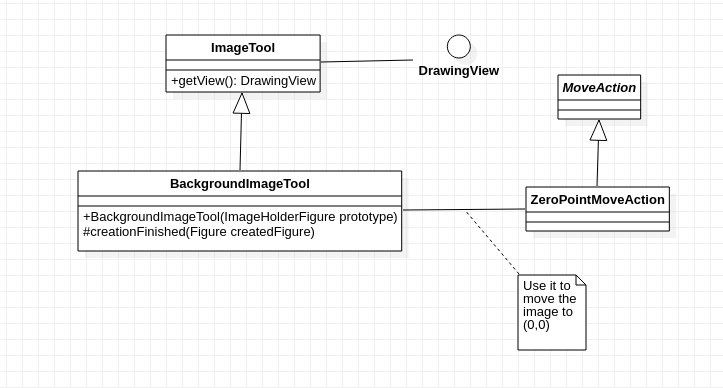
\includegraphics[keepaspectratio,width=\textwidth]{images/SketchImporter.png}
    \caption{SketchImporter Implementation}
\end{figure}
